% slides/proposed_method.tex

\begin{frame}
\frametitle{Proposed Method Overview}

\begin{itemize}
    \item Enhancing the Restorable Arbitrary Style Transfer (RAST) framework through targeted modifications.
    \item Key Contributions:
    \begin{enumerate}
        \item Ablation Study to assess the significance of various loss components.
        \item Introduction of Idempotency Loss to enforce consistent style transfer behavior.
        \item Adaptation of Multirestoration Loss tailored for low-resolution images.
        \item Architectural Simplifications to streamline the model without compromising performance.
    \end{enumerate}
\end{itemize}

\end{frame}

\begin{frame}
\frametitle{Ablation Study}

\begin{itemize}
    \item \textbf{Objective:} Determine the contribution of each loss component in the RAST framework.
    \item \textbf{Methodology:}
    \begin{itemize}
        \item Systematically remove each loss term from the total loss function.
        \item Evaluate the impact on style transfer quality and restoration capability.
    \end{itemize}
    \item \textbf{Total Loss Function:}
    \[
    \mathcal{L} = \lambda_{\text{contra}} \mathcal{L}_{\text{contra}} + \lambda_{\text{identity}} \mathcal{L}_{\text{identity}} + \lambda_{\text{diff}} \mathcal{L}^{-1}_{\text{diff}} + \lambda_{\text{multi}} \mathcal{L}_{\text{multi}} + \lambda_{\text{adv}} \mathcal{L}_{\text{adv}}
    \]
    \begin{itemize}
        \item \(\mathcal{L}_{\text{contra}}\): Contrastive Loss
        \item \(\mathcal{L}_{\text{identity}}\): Identity Loss
        \item \(\mathcal{L}^{-1}_{\text{diff}}\): Style Difference Loss
        \item \(\mathcal{L}_{\text{multi}}\): Multi-Restoration Loss
        \item \(\mathcal{L}_{\text{adv}}\): Adversarial Loss
    \end{itemize}
\end{itemize}

\end{frame}

\begin{frame}
\frametitle{Ablation Study Results}

\begin{itemize}
    \item \textbf{Findings:}
    \begin{itemize}
        \item Each loss component significantly contributes to the overall performance.
        \item Removal of the Multi-Restoration Loss leads to a notable decline in restoration quality.
    \end{itemize}
    \item \textbf{Visual Impact:}
    \begin{figure}[H]
        \centering
        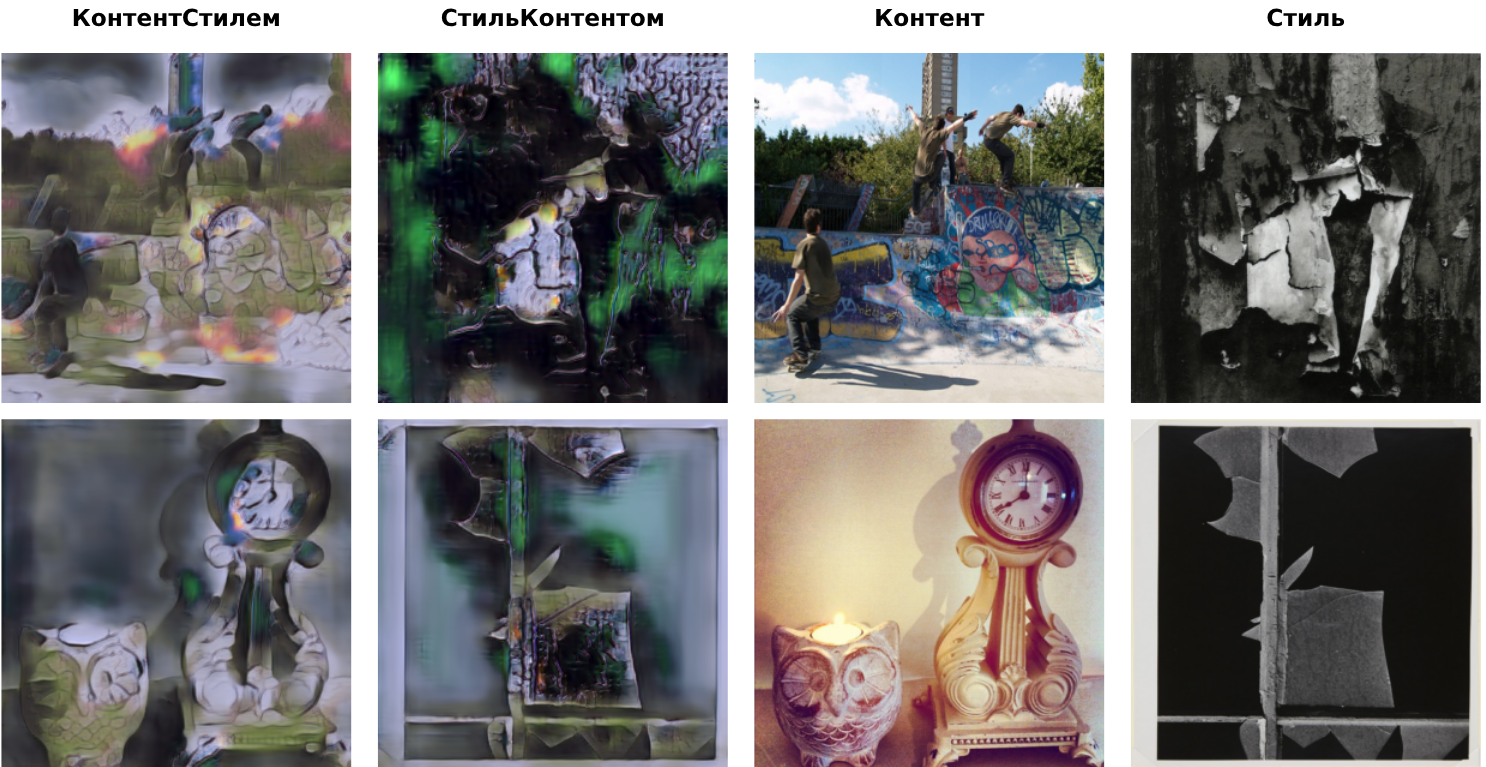
\includegraphics[width=0.7\textwidth]{figures/ablation_results.png}
        \caption{Effect of Removing Multi-Restoration Loss}
        \label{fig:ablation}
    \end{figure}
\end{itemize}

\end{frame}

\begin{frame}
\frametitle{Idempotency Loss}

\begin{itemize}
    \item \textbf{Purpose:} Ensure consistent stylization results when the style transfer operation is applied multiple times.
    \item \textbf{Mathematical Formulation:}
    \[
    T(T(I_c, I_s), I_s) = T(I_c, I_s)
    \]
    \[
    \mathcal{L}_{\text{idemp}} = \| T(T(I_c, I_s), I_s) - T(I_c, I_s) \|^2
    \]
    \begin{itemize}
        \item \(T\): Style Transfer Operation
        \item \(I_c\): Content Image
        \item \(I_s\): Style Image
    \end{itemize}
    \item \textbf{Implementation:}
    \begin{itemize}
        \item Adds a constraint that the output remains unchanged upon repeated applications of the same style.
    \end{itemize}
\end{itemize}

\end{frame}

\begin{frame}
\frametitle{Idempotency Loss Impact}

\begin{itemize}
    \item \textbf{Evaluation:}
    \begin{itemize}
        \item Compare stylization results with and without Idempotency Loss.
        \item Apply style transfer operation twice on the same content and style images.
    \end{itemize}
    \item \textbf{Results:}
    \begin{itemize}
        \item \textbf{With \( \mathcal{L}_{\text{idemp}} \):} Consistent stylized images upon repeated applications.
        \item \textbf{Without \( \mathcal{L}_{\text{idemp}} \):} Subtle changes in style intensity and minor artifacts upon multiple applications.
    \end{itemize}
\end{itemize}   

\end{frame}

\begin{frame}
\frametitle{Idempotency Loss Impact}

\begin{figure}[H]
    \centering
    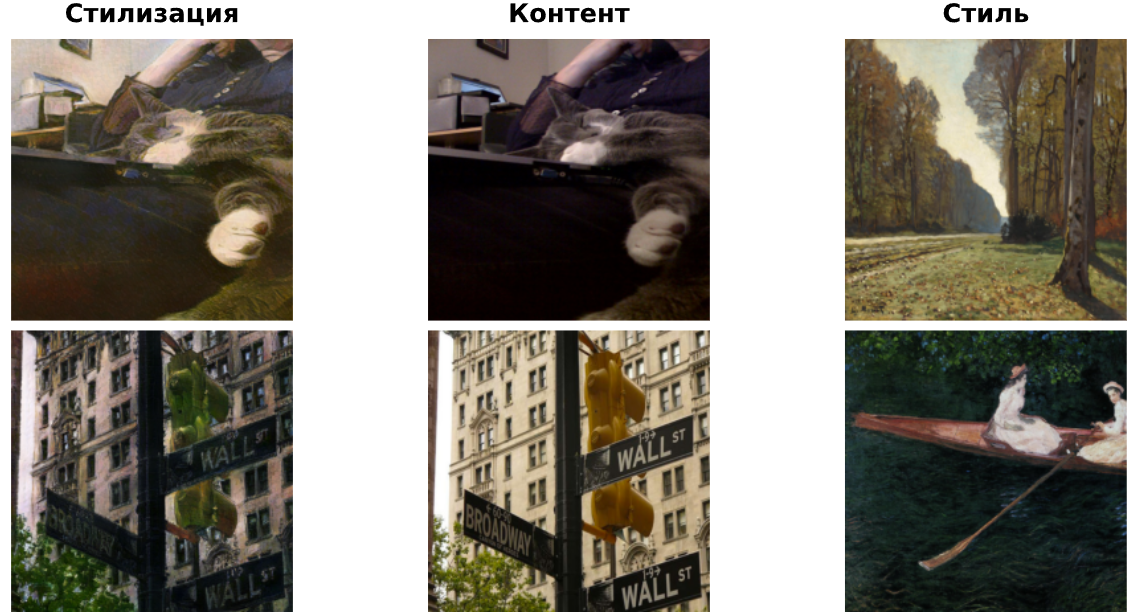
\includegraphics[width=0.7\textwidth]{figures/idempotency.png}
    \caption{Stylization with Idempotency Loss (\( \mathcal{L}_{\text{idemp}} \))}
    \label{fig:idempotency_result}
\end{figure}

\end{frame}

\begin{frame}
\frametitle{Idempotency Loss Impact}
\begin{figure}[H]
    \centering
    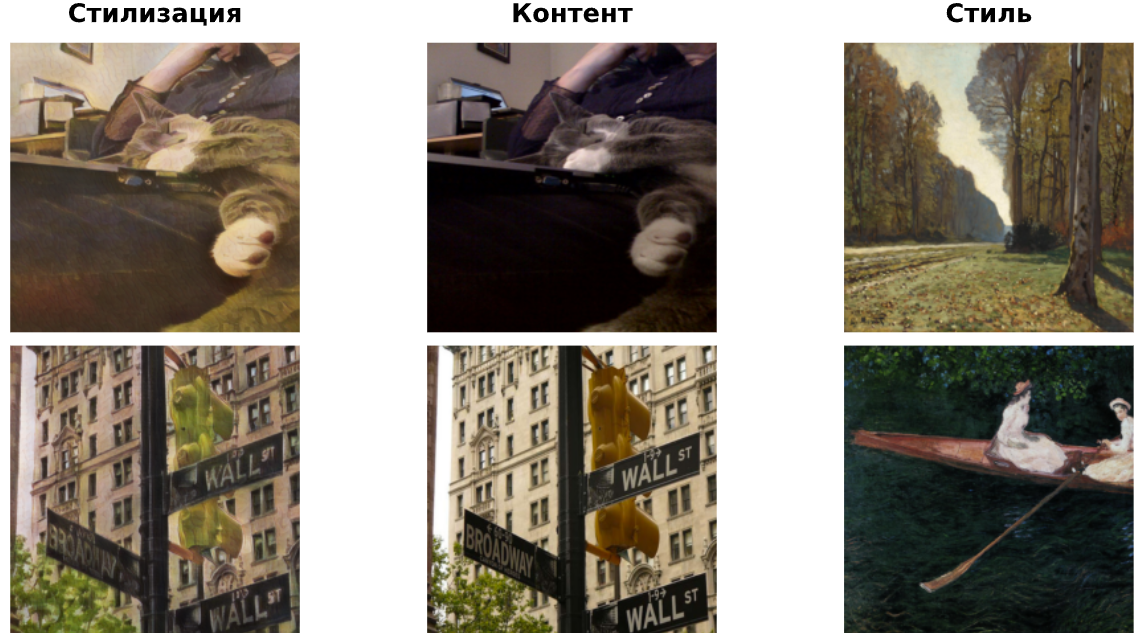
\includegraphics[width=0.7\textwidth]{figures/without_idempotency.png}
    \caption{Stylization without Idempotency Loss}
    \label{fig:without_idempotency_result}
\end{figure}
\end{frame}

\begin{frame}
\frametitle{Multirestoration Loss for Low-Resolution Images}

\begin{itemize}
    \item \textbf{Challenge:} Standard Multi-Restoration Loss leads to excessive colorization in low-resolution images, degrading style transfer quality.
    \item \textbf{Proposed Solution:}
    \begin{itemize}
        \item Adapt the Multi-Restoration Loss to better handle low-resolution scenarios.
        \item Incorporate a weighting mechanism to emphasize restoration accuracy at lower resolutions.
    \end{itemize}
    \item \textbf{Mathematical Formulation:}
    \[
    \mathcal{L}_{\text{multi\_low\_res}} = \mathcal{L}_{\text{multi}}(\text{LowRes}(I_c), \text{LowRes}(I_c))
    \]
    \begin{itemize}
        \item \( \text{LowRes} \): Function to obtain low-resolution representations.
    \end{itemize}
    \item \textbf{Outcome:} Aims to maintain color distribution and visual fidelity without over-altering colors.
\end{itemize}

\end{frame}

\begin{frame}
\frametitle{Multirestoration Loss Impact on Low-Resolution Images}

\begin{itemize}
    \item \textbf{Evaluation:}
    \begin{itemize}
        \item Conduct experiments on images resized to \(32 \times 32\) pixels.
    \end{itemize}
    \item \textbf{Results:}
    \begin{itemize}
        \item \textbf{Performance:} Both baseline and enhanced models perform poorly on low-resolution images.
        \item \textbf{Issues:} Noticeable artifacts and significant color deviations; stylized outputs lack detail and coherence.
    \end{itemize}
\end{itemize}
\end{frame}

\begin{frame}
\frametitle{Multirestoration Loss Impact on Low-Resolution Images}
\begin{figure}[H]
    \centering
    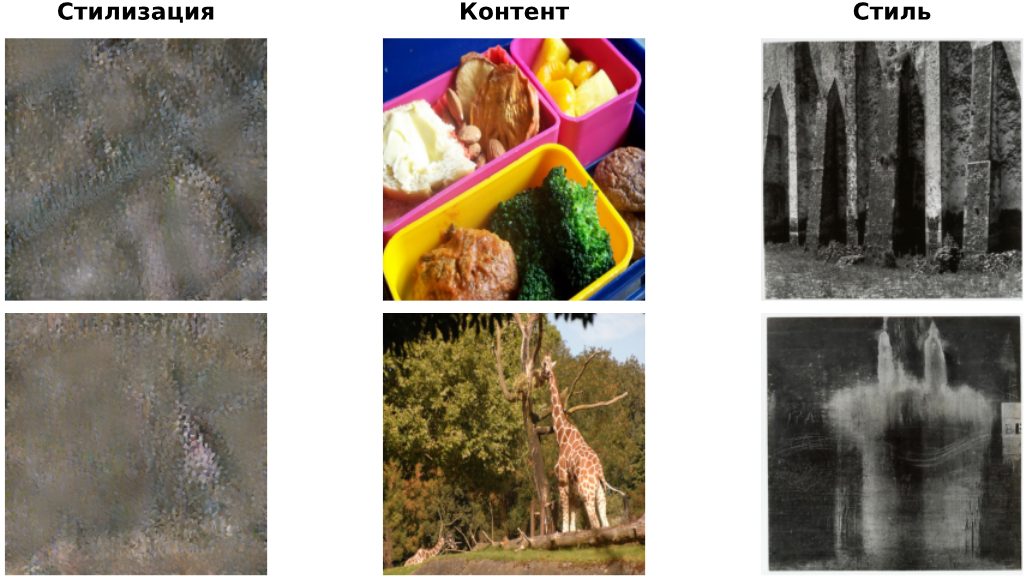
\includegraphics[width=0.7\textwidth]{figures/lowres.png}
    \caption{Stylization and Restoration on Low-Resolution Images (\(32 \times 32\) pixels)}
    \label{fig:lowres_results}
\end{figure}
\end{frame}

\begin{frame}
\frametitle{Architectural Simplification}

\begin{itemize}
    \item \textbf{Objective:} Assess the impact of simplifying the RAST architecture by removing non-essential components.
    \item \textbf{Approach:}
    \begin{itemize}
        \item Retain only core modules responsible for style transfer and restoration.
        \item Replace encoder module with pretrained EfficientNet \cite{tan2020efficientnetrethinkingmodelscaling}.
    \end{itemize}
    \item \textbf{Findings:}
    \begin{itemize}
        \item \textbf{Performance Degradation:} Simplified model exhibits poorer stylization results.
        \item \textbf{Efficiency vs. Quality:} While the model is lighter, the quality of style transfer is adversely affected.
    \end{itemize}
    \item \textbf{Conclusion:}
    \begin{itemize}
        \item Certain architectural components are critical for maintaining high-quality style transfer.
        \item Simplifications may introduce inefficiencies and degrade performance.
    \end{itemize}
\end{itemize}

\end{frame}

\begin{frame}
\frametitle{Overall Objective Function}

\begin{itemize}
    \item \textbf{Combined Objective:}
    \[
    \mathcal{L} = \lambda_{\text{contra}} \mathcal{L}_{\text{contra}} + \lambda_{\text{identity}} \mathcal{L}_{\text{identity}} + \lambda_{\text{diff}} \mathcal{L}^{-1}_{\text{diff}} +
    \]
    \[
    + \lambda_{\text{multi\_low\_res}} \mathcal{L}_{\text{multi\_low\_res}} + \lambda_{\text{adv}} \mathcal{L}_{\text{adv}} + \lambda_{\text{idemp}} \mathcal{L}_{\text{idemp}}
    \]
    \begin{itemize}
        \item \textbf{Purpose:} Balances contributions of each loss component during training.
        \item \textbf{Impact:} Ensures that all aspects of style transfer and restoration are adequately addressed.
    \end{itemize}
\end{itemize}

\end{frame}
